% Chapter Template

\chapter{Experiments and results} % Main chapter title

\label{Chapter9} % Change X to a consecutive number; for referencing this chapter elsewhere, use \ref{ChapterX}

In this chapter the most relevant experiments done are explained.\\\\\\
All these experiments were done on a laptop with the following characteristics:
\begin{itemize}
	\item 8 GB of RAM
	\item Intel® Core™ i7-4500U CPU @ 1.80GHz × 4 
	\item Ubuntu 16.04 LTS
\end{itemize}

\section{Encoding Boolean formulas to CNF}

The goal of this experiment was trying to find the best value to decide which type of encoding use to convert Boolean formulas into CNFs. This value represent the portion of 1s function's primes cover. If the portion is small enough, then a lot of clauses are generated.\\
To do that, some Boolean formulas were randomly generated and some portion values between 0,0001 and 1 were tried.\\
For each value, the number of variables and clauses of the generated CNFs were stored.

\begin{center}
	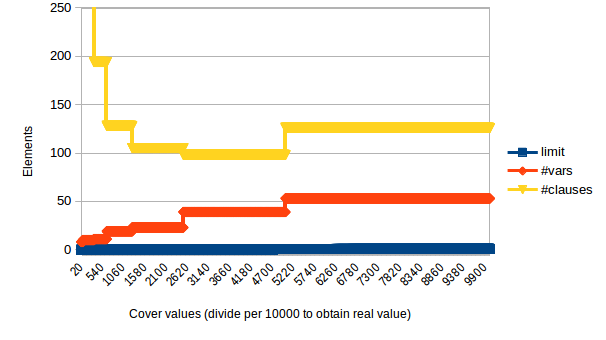
\includegraphics[width=0.8\textwidth]{Figures/value-cover.png}
	\captionof{figure}{Number of clauses and variables for each portion value}
	\label{value-cover}
\end{center}
As the reader can see in the figure above [\ref{value-cover}], the number of clauses rapidly decreases because of the addition of new variables.\\
Between 2620 and 5220, the CNFs were generated with the minimum number of clauses, i.e. the recommended portion is one between 0,262 and 0,522.

\section{Pseudo-Boolean Minimisation benchmarks}

The goal of this experiment was to compare the time required to solve Pseudo-Boolean minimisation problems with \emph{Linear search} and \emph{Binary search}.\\
The International Center for Computational Logic\footnote{http://pbeva.computational-logic.org/} has available some benchmarks from their previous competitions, in particular, MINLPLIB2 which offers Pseudo-Boolean optimisation problems. \\\\
From that problems, four of them were selected:
\begin{itemize}
	\item minlplib2-pb-0.1.0/opb/autocorr\_bern20-03.opb\\ variable= 20 constraint= 1 product= 18 sizeproduct= 36
	\item minlplib2-pb-0.1.0/opb/hmittelman.opb\\ variable= 16 constraint= 7 product= 9 sizeproduct= 44
	\item minlplib2-pb-0.1.0/opb/sporttournament10.opb\\ variable= 45 constraint= 1 product= 80 sizeproduct= 160
	\item minlplib2-pb-0.1.0/opb/crossdock\_15x7.opb\\ variable= 210 constraint= 44 product= 2793 sizeproduct= 5586
\end{itemize}
To convert these benchmarks to a syntax which could be understood by the software, a python script was made.
\begin{itemize}
	\item The constraints and the cost function were not linear, i.e. of the form $w_1 v_1 v_2 + w_2 v_2 v_3 \geq k$. These expressions were simplified keeping only the first variable of each term: $w_1 v_1+ w_2 v_2 \geq k$ 
	\item The relational operator in the constraints was $\geq$. These were converted to equivalent constraints with $\leq$. To do that, the script negated all the weights. 
\end{itemize}
For each benchmark, two files were created: one using the Linear search algorithm and the other using Binary search algorithm.\\
For minlplib2-pb-0.1.0/opb/autocorr\_bern20-03.opb:
\begin{itemize}
	\item benchmarks\_files/bench\_1\_bin.cpp
	\item benchmarks\_files/bench\_1\_lin.cpp
\end{itemize}
For minlplib2-pb-0.1.0/opb/hmittelman.opb:
\begin{itemize}
	\item benchmarks\_files/bench\_2\_bin.cpp
	\item benchmarks\_files/bench\_2\_lin.cpp
\end{itemize}
For minlplib2-pb-0.1.0/opb/sporttournament10.opb:
\begin{itemize}
	\item benchmarks\_files/bench\_3\_bin.cpp
	\item benchmarks\_files/bench\_3\_lin.cpp
\end{itemize}
For minlplib2-pb-0.1.0/opb/crossdock\_15x7.opb:
\begin{itemize}
	\item benchmarks\_files/bench\_4\_bin.cpp
	\item benchmarks\_files/bench\_4\_lin.cpp
\end{itemize}


\begin{center}
	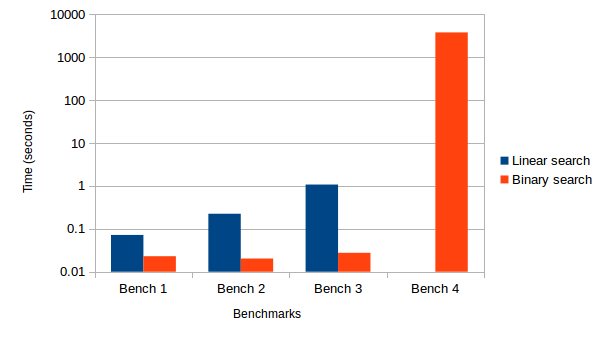
\includegraphics[width=0.8\textwidth]{Figures/benchmarks.png}
	\captionof{figure}{Time per search algorithm for each benchmark}
	\label{benchmark}
\end{center}
As the reader can see in the figure above [\ref{benchmark}], in all the benchmarks Binary search was faster than Linear search. In the last one, Binary search took 3.77,62 seconds (1,05 h), whereas Linear search did not end after 8 hours of execution. That is the reason why it is not represented.\\\\
However, even that Linear search is slower than Binary search, its cost function encoding into CNF using Incremental Constraints was considerably faster than the conventional encoding used in Binary search. 